\documentclass[10pt]{article}

\usepackage[margin=2cm]{geometry}
\usepackage[backend=biber]{biblatex}
\usepackage{multicol}
\usepackage{caption}
\usepackage{tikz}
\usepackage{hyperref}
\usepackage{listings}
\usepackage{color}
\usepackage{xcolor}

\lstdefinelanguage{JavaScript}{
  keywords={break, case, catch, continue, debugger, default, delete, do, else, false, finally, for, function, if, in, instanceof, new, null, return, switch, this, throw, true, try, typeof, var, void, while, with},
  morecomment=[l]{//},
  morecomment=[s]{/*}{*/},
  morestring=[b]',
  morestring=[b]",
  ndkeywords={class, export, boolean, throw, implements, import, this},
  keywordstyle=\color{blue}\bfseries,
  ndkeywordstyle=\color{darkgray}\bfseries,
  identifierstyle=\color{black},
  commentstyle=\color{purple}\ttfamily,
  stringstyle=\color{red}\ttfamily,
  sensitive=true
}

\newenvironment{Figure}
  {\par\medskip\noindent\minipage{\linewidth}}
  {\endminipage\par\medskip}

\addbibresource{refs.bib}

\begin{document}

\pagenumbering{gobble}

\begin{center}
{\bf ENGINEERING TRIPOS PART II B} \\
\vspace{0.2cm}
{\bf 4B25 PROJECT REPORT \hfill 17/1/19 \hfill Harry Sarson}
\vspace{0.2cm}
\rule{15.7cm}{0.5mm}
\end{center}

\begin{multicols}{2}

The RISC-V REPL is a Read Eval Print Loop for RISC-V - an open source Instruction Set Architecture (ISA)\cite{riscv-homepage} - hosted at github.com/harrysarson/riscv-repl.

This project allows execution of individual RISC-V instructions via a terminal application.
When an instruction is entered, it is compiled into machine code which is sent via UART to an FPGA where it is executed.
Once the FPGA has executed the instruction it sends the register file back over UART where is it displayed in the console.

\section{State of the Art}

Assembly REPL's which allow execution of native instructions can be found online.
\href{https://github.com/yrp604/rappel}{rappel} supports linux systems whilst Windows uses can use \href{https://github.com/zerosum0x0/WinREPL}{WinREPL}.
Both use similar approaches, creating a separate process and editing the binary whilst it is running.
The instructions entered are (after assembling) run directly by the processor.

Additionally, RISC-V emulators such as \href{https://bellard.org/tinyemu/}{tinyemu} or the \href{https://github.com/phillipstanleymarbell/sunflower-simulator}{sunflower-simulator} allow RISC-V programs to be run on a desktop computer by simulating execution of the instructions in software\cite{tinyemu}\cite{sunflower}.

RISC-V processors have been written in verilog with the aim of running on an FPGA, two examples are \href{https://github.com/cliffordwolf/picorv32}{PicoRV32} and \href{https://github.com/physical-computation/RV32I_iCE40}{RV32I\_iCE40}\cite{picorv32}\cite{RV32I_iCE40}.

\section{Approach}

To create the RISC-V REPL I chose to use the RV32I\_iCE40 verilog modules as they are designed to run on the same FPGA (the iCE40 Ultra Plus) and because I knew I could seek help from Ryan Voo to get started.

RV32I\_iCE40 has support for transmitting bytes over UART from software using memory mapped registers.
As UART would be used for loading instructions and writing back the register file, the ability to write to UART from software was removed.
Additionally, modules to receive bytes over UART were added into the project.
The modules were sourced from \href{https://github.com/FPGAwars/FPGA-peripherals}{FPGA-peripherals} - the same place as the transmitting modules already included\cite{FPGA-peripherals}.

When not executing an instruction, the processor clock is held high.
Then, once an instruction is received, that instruction is sent to the processor and the processor clock is made to complete one cycle.
The processor has a five stage pipeline and thus four more cycles are required to fully execute the instruction.
The clock cycled four more times whilst no-op instructions are sent to the processor.
Finally, the register file is read and transmitted.
Figure \ref{fig:timing} shows a timing diagram of this process.

Further technical details can be found in the documentation directory of the RISC-V REPL repository.

\section{Running in Simulation}

During this project \href{https://www.veripool.org/wiki/verilator}{verilator} was used to test the design.
Verilator is a verilog to c++ compiler and by running of the processor in a software testbed, debugging information can be printed to the terminal.
Additionally, compiling the simulations is much faster than synthesizing a hardware layout and flashing to an FPGA.
The simulation allows connecting the FPGA UART to a TCP port, this is used to connect the user interface to the processor when it is running in simulation.

Moreover, the iCE40 Ultra Plus FPGA used in this coursework contains a limited number of resources.
Figure \ref{fig:lcs} shows that the current implementation of the RISC-V REPL processor requires more logic cells than the FPGA has available.
It is likely that a better HDL implementation of the processor would be able to cut down the number of logic cells needed.
The method of writing the register file is particularly clunky - a 1014 bit vector wire is assigned to the bits of the registers and this vector is transmitted one byte at a time over UART.
Unfortunately, efforts to reduce the number of logic cells required were fruitless and, due to time constraints, were abandoned.
With a better understanding of verilog and some more time, it is believed that a synthesizable version could be obtained.

\begin{Figure}
  \centering
  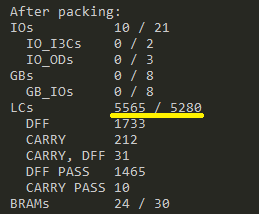
\includegraphics[width=0.7\textwidth]{../images/fpga-resources.png}
  \captionof{figure}{The synthesis requires more logic cells than are avaiable.\cite{wavedrom}}
  \label{fig:lcs}
\end{Figure}

\section{REPL User Interface}

The processor provides an UART interface, this project includes a terminal application written using \href{https://nodejs.org}{Node.js}.
I chose to use node as I knew I could use the \verb|serialport| package to interface with the FPGA.

The user interface must assemble RISC-V instructions into machine code.
To use gcc as a RISC-V assembler it must be built as a cross compiler which was done by including the Sunflower-toolchain as part of this project\cite{sunflower}.
Instructions entered into the REPL can be converted into a valid assembly file as shown in listing \ref{lst:make-assembly}.

\begin{lstlisting}[
    language=JavaScript,
    upquote=true,
    frame = single,
    caption={Create assembly from single instruction.},
    label={lst:make-assembly}]
const createAssembly = instruction => `
.globl _start

_start:
	${instruction}
`;
\end{lstlisting}

A small Makefile uses the cross compiler to generate both machine code and disassembly from an assembly file.
My node script reads an instruction from the terminal, converts it into an assembly file, writes this file to disk, executes \verb|make| and finally reads the disassembly and machine code from the disk.
The disassembly is displayed to the user and the machine code is sent to the processor.
As figure \ref{fig:invalid-inst} shows, if the user enters invalid RISC-V assembly, then the error message generated by gcc is shown to the user.

\begin{Figure}
  \centering
  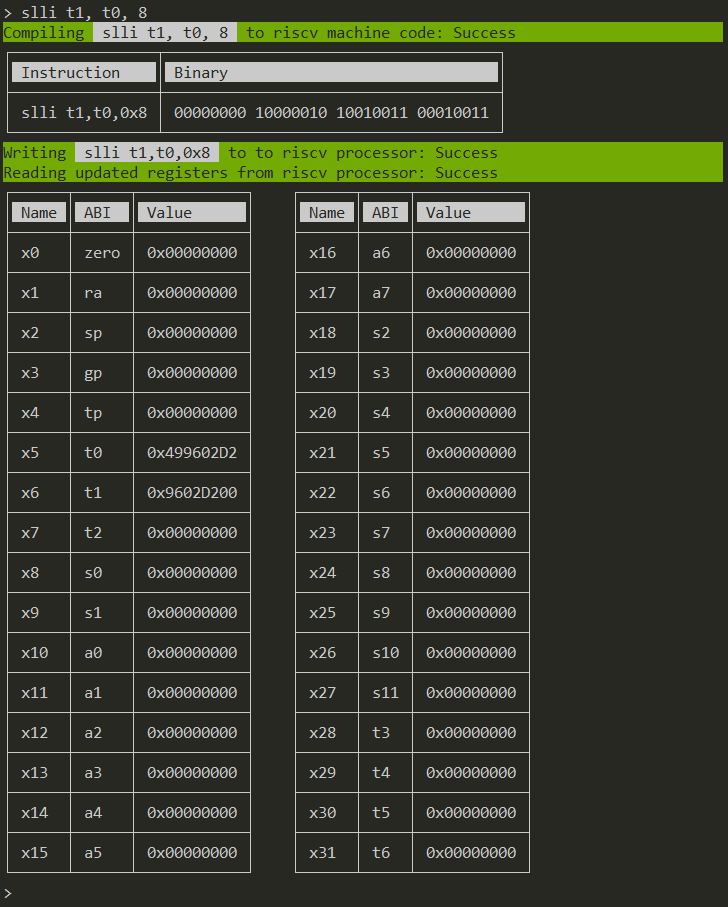
\includegraphics[width=0.9\textwidth]{../images/slli-screenshot.png}
  \captionof{figure}{Screenshot of RISC-V REPL showing execution of the logical shift left immediate instruction.}
\end{Figure}


\end{multicols}

\begin{Figure}
  \centering
  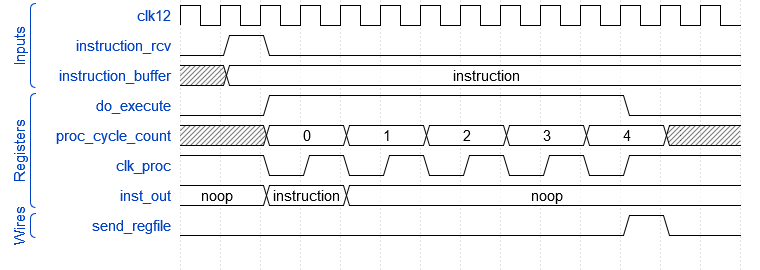
\includegraphics[width=0.9\textwidth]{../images/timing-diagram.png}
  \captionof{figure}{Timing diagram, the processor clock (clk\_proc) cycles five times to pass the instruction though the pipeline. inst\_out is the instruction fetched by the processor at each rising edge of the processor clock.\cite{wavedrom}}
  \label{fig:timing}
\end{Figure}

\begin{Figure}
  \centering
  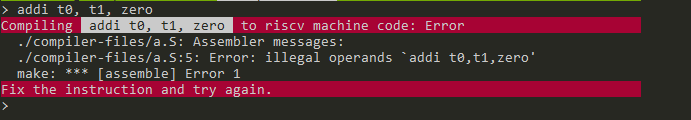
\includegraphics[width=\textwidth]{../images/invalid-instr.png}
  \captionof{figure}{Error generated when an invalid instruction is entered.}
  \label{fig:invalid-inst}
\end{Figure}

\printbibliography

\end{document}

